\documentclass{beamer}

\mode<presentation> {
\usetheme{Boadilla}
\usecolortheme{default}
\usefonttheme[onlymath]{serif}
}
\usepackage{amsmath}
\usepackage{amssymb}
\usepackage{amsthm}

\usepackage{caption}
\usepackage{hyperref}
\usepackage{booktabs}
\usepackage{array} 
\usepackage{filecontents}
\usepackage{pgfplots, pgfplotstable}

\pgfplotsset{compat=1.16}
\usepackage[USenglish,british,american,australian,english]{babel}
\begin{filecontents}{\jobname.bib}
@article{qian1999momentum,
  title={On the momentum term in gradient descent learning algorithms},
  author={Qian, Ning},
  journal={Neural networks},
  volume={12},
  number={1},
  pages={145--151},
  year={1999},
  publisher={Elsevier}
}

@article{duchi2011adaptive,
  title={Adaptive subgradient methods for online learning and stochastic optimization.},
  author={Duchi, John and Hazan, Elad and Singer, Yoram},
  journal={Journal of machine learning research},
  volume={12},
  number={7},
  year={2011}
}

@article{ruder2016overview,
  title={An overview of gradient descent optimization algorithms},
  author={Ruder, Sebastian},
  journal={arXiv preprint arXiv:1609.04747},
  year={2016}
}

@software{Novik_torchoptimizers,
    title        = {{torch-optimizer -- collection of optimization algorithms for PyTorch.}},
    author       = {Novik, Mykola},
    year         = 2020,
    month        = 1,
    version      = {1.0.1}
}

\end{filecontents}
\usepackage[style=numeric,backend=biber,autocite=plain,sorting=none]{biblatex}
\addbibresource{\jobname.bib}
  
\usepackage{graphicx} % Allows including images

\usepackage{booktabs} % Allows the use of \toprule, 
\usepackage{listings}
\usepackage{minted}
\usepackage{tikz}
%\usepackage{etoolbox} % for \ifthen
\usepackage{listofitems} % for \readlist to create arrays
\usetikzlibrary{datavisualization, arrows.meta} % for arrow size
\usepackage[outline]{contour} % glow around text
\contourlength{1.4pt}

\tikzset{>=latex} % for LaTeX arrow head
\usepackage{xcolor}

% Scientific libs


\def\nstyle{int(\lay<\Nnodlen?min(2,\lay):3)} % map layer number onto 1, 2, or 3
\DeclareMathOperator*{\argmax}{arg\,max}
\DeclareMathOperator*{\argmin}{arg\,min}
\setbeamertemplate{caption}[numbered]
\AtBeginBibliography{\small}

%Includes "References" in the table of contents

\title[CodeSeoul] % (optional, only for long titles)
  {Dimensionality reduction techniques}

\author[Machine Learning Afternoons] % (optional, for multiple authors)
  {Sanzhar Askaruly (San)}

\institute[] % (optional)
  { Ulsan National Institute of Science and Technology\newline
    Ph.D. Candidate in Biomedical Engineering}

\date[December 10]
{CodeSeoul MLA \\December 10, 2022}

% some change
\begin{document}
    %\maketitle
    \begin{frame}
    \titlepage % Print the title page as the first slide
    \end{frame}

    \begin{frame}{Overview}
      What we'll cover today:
      \tableofcontents
    \end{frame}
    
    \section{Motivation} %
    \begin{frame}{Motivation}
        \begin{itemize}
            \item Relationships between data
        \end{itemize}
    \end{frame}

    \section{Background mathematics}
    \begin{frame}
        \frametitle{Population vs sample}
        \begin{center}
            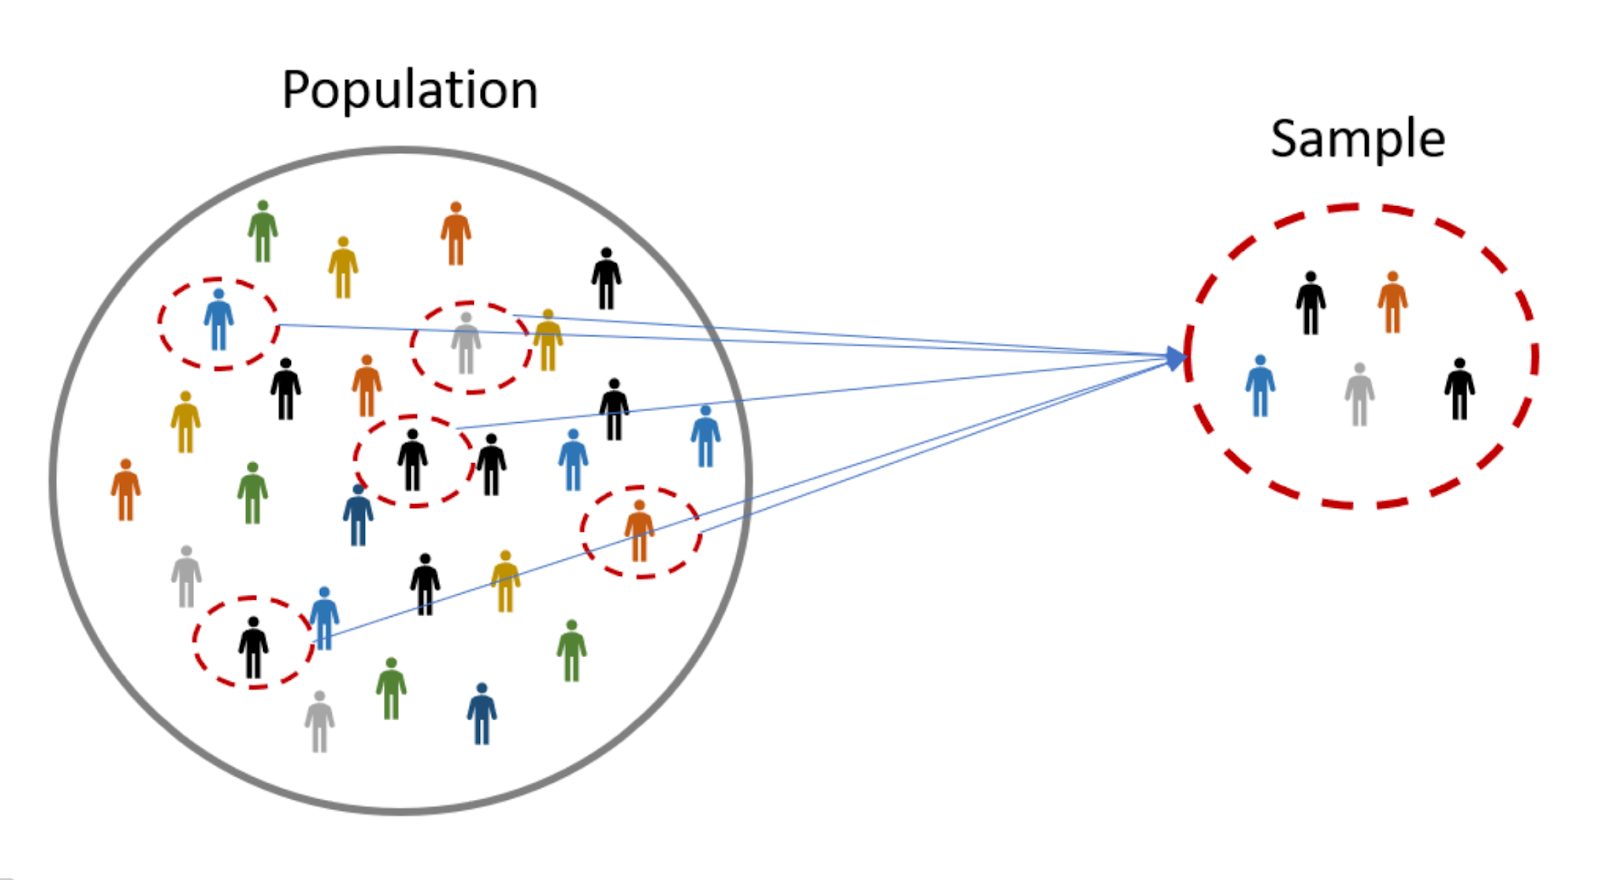
\includegraphics[width=0.9\textwidth]{/home/suzy/gitrepos/tuttelikz/machine-learning/221210-pca/images/sample_vs_population.png}
        \end{center}
    \end{frame}

    \subsection{Sample mean}
    \begin{frame}
        \frametitle{Population vs sample}
        \begin{columns}
            \begin{column}{0.4\textwidth}  %%<--- here
                \begin{center}
                    \begin{block}{Population mean}
                        
                        \begin{equation}    % <--- deleted empty lines
                            \mu = \frac{\sum_{i=1}^N x_i}{N}
                        \end{equation}

                        $N$ is number of items in the population
                    \end{block}
                \end{center}
            \end{column}
            \begin{column}{0.4\textwidth}  %%<--- here
                \begin{center}
                    \begin{block}{Sample mean}
                        
                        \begin{equation}    % <--- deleted empty lines
                            \bar{{X}} = \frac{\sum_{i=1}^n x_i}{n}
                        \end{equation}
                        $n$ is number of items in the sample
                    \end{block}
                \end{center}
            \end{column}
        \end{columns}
    \end{frame}    
    
    \subsection{Standard deviation}
    \begin{frame}[fragile]
        \frametitle{Standard deviation}
        Let's take a look on two samples:\\~\\
        \begin{center}$A = \left[ 10\: 20\: 40\: 70 \right]$\end{center}
        \begin{center}
            
            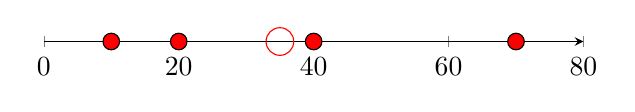
\begin{tikzpicture}
                \begin{axis}[
                    xmin=0, xmax=80,
                    axis x line=bottom,% only show the bottom x axis
                    hide y axis,    
                    ymin=0,ymax=1,
                    scatter/classes={%
                        a={mark=o,draw=black}}
                    ]
                
                \addplot[scatter,only marks,
                    mark size = 3pt,
                    fill = red,
                    scatter src=explicit symbolic]
                table {
                    10 0 
                    20 0 
                    40 0 
                    70 0 
                };
                \addplot[scatter,only marks,
                    mark size = 5pt,
                    mark=o,red,
                    scatter src=explicit symbolic]
                table {
                    35 0 
                };
                \end{axis}
                
            \end{tikzpicture}
        \end{center}
        
        \begin{center}$B = \left[ 30\: 33\: 37\: 40 \right]$\end{center}
        \begin{center}
            
            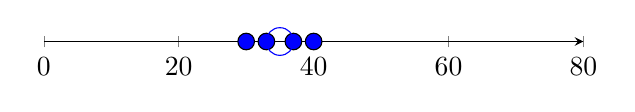
\begin{tikzpicture}
                \begin{axis}[
                    xmin=0, xmax=80,
                    axis x line=bottom,% only show the bottom x axis
                    hide y axis,    
                    ymin=0,ymax=1,
                    scatter/classes={%
                        a={mark=o,draw=black}}
                    ]
                
                \addplot[scatter,only marks,
                    mark size = 3pt,
                    fill = blue,
                    scatter src=explicit symbolic]
                table {
                    30 0 
                    33 0 
                    37 0 
                    40 0 
                };
                \addplot[scatter,only marks,
                    mark size = 5pt,
                    mark=o,blue,
                    scatter src=explicit symbolic]
                table {
                    35 0 
                };
                \end{axis}
                
            \end{tikzpicture}
        \end{center}
        Here, $\bar{{A}} = \bar{{B}} = 35$. Unfortunately, mean doesn't tell us a lot except for a middle point.
    \end{frame}

    \begin{frame}
        \frametitle{Standard deviation}
        For our two sets, $A = \left[ 10\: 20\: 40\: 70 \right]$ and $B = \left[ 30\: 33\: 37\: 40 \right]$, we would be more interested in the \emph{spread} of the data.
        \bigskip
        So, how do we calculate it?
        \begin{center}    
            \begin{block}{Standard deviation}
                \begin{equation}    % <--- deleted empty lines
                    s = \sqrt{\frac{\sum_{i=1}^n (X_i - \bar{X})^2}{(n-1)}}
                \end{equation}
                In plain English, it is the "average distance from the mean of the data set to a point."
            \end{block}
        \end{center}
        
    \end{frame}

    \begin{frame}[fragile]
        \frametitle{Standard deviation}
        Set 1: $A = \left[ 10\: 20\: 40\: 70 \right]$, and $\bar{A}=35$
        \begin{center}
            
            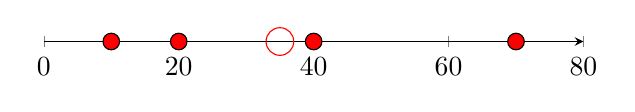
\begin{tikzpicture}
                \begin{axis}[
                    xmin=0, xmax=80,
                    axis x line=bottom,% only show the bottom x axis
                    hide y axis,    
                    ymin=0,ymax=1,
                    scatter/classes={%
                        a={mark=o,draw=black}}
                    ]
                
                \addplot[scatter,only marks,
                    mark size = 3pt,
                    fill = red,
                    scatter src=explicit symbolic]
                table {
                    10 0 
                    20 0 
                    40 0 
                    70 0 
                };
                \addplot[scatter,only marks,
                    mark size = 5pt,
                    mark=o,red,
                    scatter src=explicit symbolic]
                table {
                    35 0 
                };
                \end{axis}
                
            \end{tikzpicture}
        \end{center}
        Let's calculate standard deviation:
        \begin{center}
            \begin{tabular}{lrr}
                \firsthline
                $A$    & $(A-\bar{A})$ & $(A-\bar{A})^2$ \\
                \hline
                10      & -25    & 625      \\
                20        & -15        & 225       \\
                40       & 5     & 25      \\
                70       & 35     & 1,225      \\
                Total       &      &  2,100     \\
                Divided by (n-1)       &      & 700   \\
                Square root       &      & \textbf{26.4575}   \\
                \lasthline
                \end{tabular}
        \end{center}

    \end{frame}

    \begin{frame}[fragile]
        \frametitle{Standard deviation}
        Set 2: $B = \left[ 30\: 33\: 37\: 40 \right]$, and $\bar{B}=35$
        \begin{center}
            
            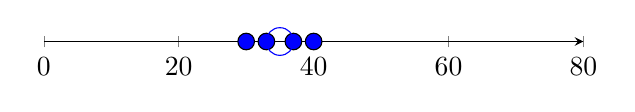
\begin{tikzpicture}
                \begin{axis}[
                    xmin=0, xmax=80,
                    axis x line=bottom,% only show the bottom x axis
                    hide y axis,    
                    ymin=0,ymax=1,
                    scatter/classes={%
                        a={mark=o,draw=black}}
                    ]
                
                \addplot[scatter,only marks,
                    mark size = 3pt,
                    fill = blue,
                    scatter src=explicit symbolic]
                table {
                    30 0 
                    33 0 
                    37 0 
                    40 0 
                };
                \addplot[scatter,only marks,
                    mark size = 5pt,
                    mark=o,blue,
                    scatter src=explicit symbolic]
                table {
                    35 0 
                };
                \end{axis}
                
            \end{tikzpicture}
        \end{center}
        Let's calculate standard deviation:
        \begin{center}
            \begin{tabular}{lrr}
                \firsthline
                $B$    & $(B-\bar{B})$ & $(B-\bar{B})^2$ \\
                \hline
                30      & -5    & 25      \\
                33        & -2        & 4       \\
                37       & 2     & 4      \\
                40       & 5     & 25      \\
                Total       &      & 58      \\
                Divided by (n-1)       &      & 19.333   \\
                Square root       &      & \textbf{4.397}   \\
                \lasthline
                \end{tabular}
        \end{center}
    \end{frame}

    \subsection{Variance}
    \begin{frame}
        \frametitle{Variance}
        Similar to standard deviation
        \bigskip
        So, how do we calculate it?
        \begin{center}    
            \begin{block}{Standard deviation}
                \begin{equation}    % <--- deleted empty lines
                    s = \sqrt{\frac{\sum_{i=1}^n (X_i - \bar{X})^2}{(n-1)}}
                \end{equation}
                In plain English, it is the "average distance from the mean of the data set to a point."
            \end{block}
        \end{center}
        
    \end{frame}


    \section{Examples}
    \subsection{Iris dataset}
    \begin{frame}
        \frametitle{Iris flower dataset}
        \begin{center}
        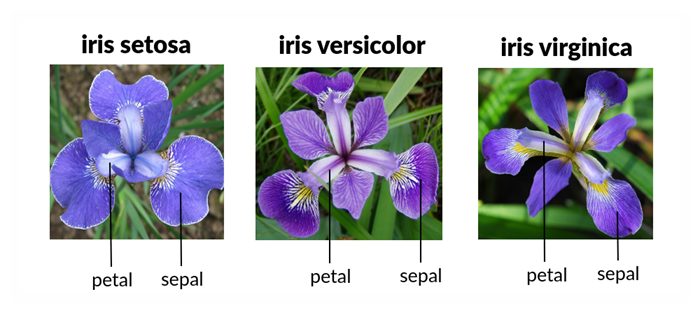
\includegraphics[width=0.9\textwidth]{/home/suzy/gitrepos/tuttelikz/machine-learning/221210-pca/images/iris.png}
        \end{center}
    \end{frame}

    
    \begin{frame}[fragile]
        \frametitle{Iris flower dataset}
        \begin{center}
        \begin{tikzpicture}[scale=0.8]
            \begin{axis}[width=6cm,height=6cm, xlabel = {Sepal length}, ylabel = {Sepal width}]
                \addplot+[scatter, only marks, scatter/classes={
                    Setosa={mark=square,red},
                    Versicolor={mark=triangle,green},
                    Virginica={mark=o,blue}}, scatter src=explicit symbolic] table[col sep=comma, header=true, x index=0, y index=1, meta index=4] {iris.csv};
                \legend{Setosa,Versicolor,Virginica},
            \end{axis}
        \end{tikzpicture}
        \hspace{1cm}
        \begin{tikzpicture}[scale=0.8]
            \begin{axis}[width=6cm,height=6cm, xlabel = {Petal length}, ylabel = {Petal width}]
                \addplot+[scatter, only marks, scatter/classes={
                    Setosa={mark=square,red},
                    Versicolor={mark=triangle,green},
                    Virginica={mark=o,blue}}, scatter src=explicit symbolic] table[col sep=comma, header=true, x index=2, y index=3, meta index=4] {iris.csv};
                \legend{Setosa,Versicolor,Virginica},
            \end{axis}
        \end{tikzpicture}
        \end{center}
        
    \end{frame}

    

    \begin{frame}
        \begin{center}
        \frametitle{Iris flower dataset}
        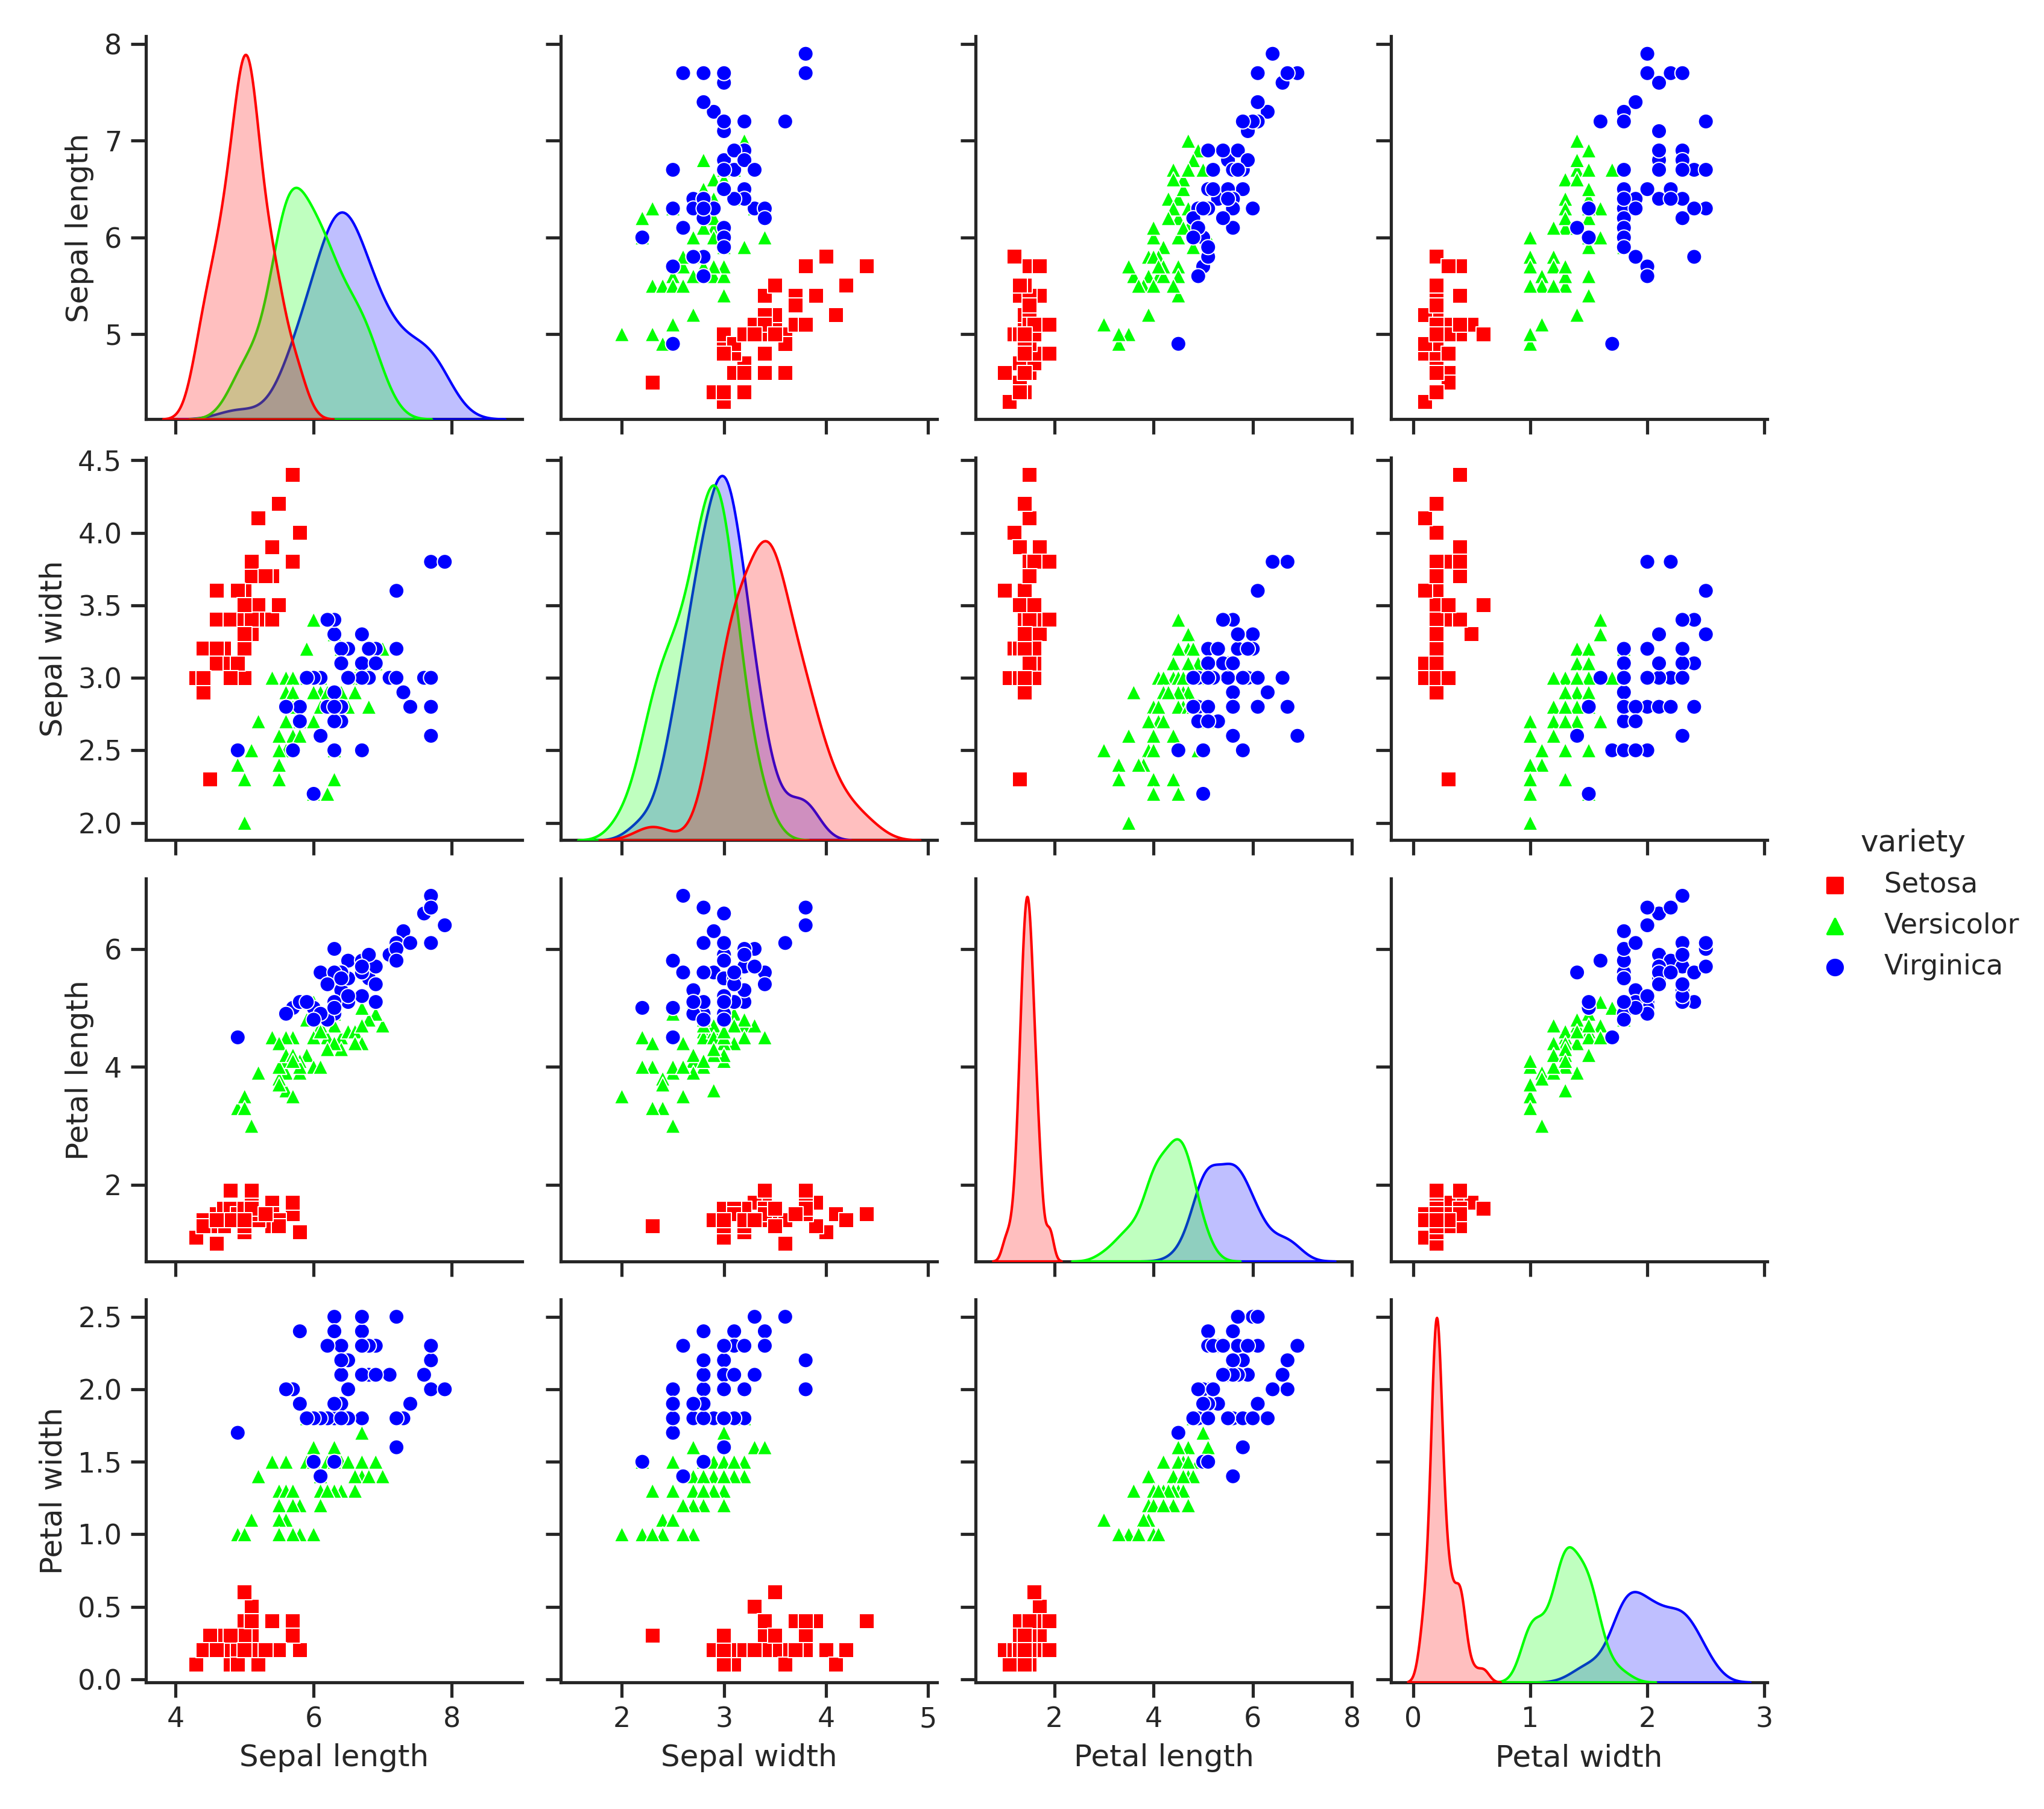
\includegraphics[width=0.7\textwidth]{/home/suzy/gitrepos/tuttelikz/machine-learning/221210-pca/images/pairplot_iris.png}
        \end{center}
    \end{frame}

    
    %mark=o,greenmark options={fill=red}

    
    \begin{frame}        
    \end{frame}

    \begin{frame}
    \end{frame}



    \begin{frame}
      \begin{center}
      \end{center}
    \end{frame}


    \begin{frame}
      \frametitle{Adagrad}
    \end{frame}


    
    \section{Experiments} %
    \begin{frame}{Experiment}
    \end{frame}
    

    \nocite{*}
    \begin{frame}{Experiment}
    \end{frame}

    \begin{frame}{Experiment}
    \end{frame}

    \begin{frame}{Experiment}
    \end{frame}
    

    \section{Summary} %
    \subsection{Conclusion}
    \begin{frame}{Conclusion}

    \end{frame}


    \subsection{Practicum}
    \begin{frame}{Practicum}
      \begin{center}
      \begin{huge}Thank you for your attention!\end{huge}
      \end{center}

        \vspace{0.5cm}
        \begin{itemize}
          \item Workshop contents: \\
            \begin{small}\url{https://github.com/CodeSeoul/machine-learning/tree/master/221210-pca}
            \end{small}
          \item Follow-up QA? \\ 
            \begin{small}\url{http://discord.com/users/tuttelikz}
            \end{small}
        \end{itemize}

    \end{frame}

    \begin{frame}{References}
      \printbibliography  
    \end{frame}

\end{document}
